BLPA: Bayesian Learn-Predict-Adjust Method for Online  Detection of Recurrent Changepoints.

\begin{abstract}
Online changepoint detection is an important task for machine learning in changing environments.
Presence of noise that can be mistaken for real changes makes it difficult to develop an effective approach that would have a low false alarm rate and being able to detect all the changes with a minimal delay.
In this paper we study how performance of popular Bayesian online detectors can be improved in case of recurrent changes. Modeling recurrence allows us to anticipate future changepoints and predict their time locations.
We propose BLPA, an efficient approach for inducing and integrating recurrence information in the streaming settings, and demonstrate its effectiveness in the experimental study on synthetic and real-world datasets.
\end{abstract}

\section{Introduction}
Online change detection is practically relevant in many domains, such as medicine, energy production, industrial processes monitoring~\cite{Nikiforov}.
In machine learning and data mining research areas change detection is often studied in the context of problem of concept drift happening due to changes in the underlying data distribution over time~\cite{Widmer96}. A popular approach for handling concept drift is to monitor data or model performance for changes and to adapt model using most recent data collected after the last detected change~\cite{GamaACMCS2014}.
%It is easier to make decisions once you are aware about the changes in a current situation.
%For a self-driving car it is important to be aware about the changes in a road condition to avoid accidents.
%If you are a user of a mobile devise equipped with a set of sensors
%changes detected in the generated data may be used to issue a recommendations to improve your health conditions or to improve your performance in a sport activity.

In this paper we consider a change detection task in a one-dimensional univariate time series data streams.
Further in the text we denote a univariate vector of observations either as $\langle x_i \rangle_{i=1}^n$ or as $\pmb{x}_{1:n}$, i.e.
\[
\pmb{x}_{1:n} \equiv \langle x_i \rangle_{i=1}^n \equiv \langle x_1, \dots, x_n \rangle
\]
Input to the change detector is a vector of observations
$\langle x_t \rangle$ indexed by the timestamps $t \in \T$.
Timestamps is an ordered vector of time moments $\T \equiv \langle t_1, \dots, t_T \rangle$ when observations were taken with a constant sampling rate.
\textit{Changepoint is a time moment when statistical properties of the data stream change significantly according to the predefined criteria.}
Changepoint is identified by the moment of time when it happened (further - `time location of the change').
%~\footnote{Further in the text the time when change has occurred is also called `time location of the change'.}.
The sequence of changes is denoted as $\Collect{c_i}_{i=1}^k \in \T$ and an individual change from this sequence as $c_i$.
Changes should be detected online when the only information observed until current moment of time can be used for an analysis.

%\subsection{Change detection problem}\label{sec:change_detection_problem}
The top plot (A) in the Fig.~\ref{fig:trellis_struct} illustrates an example of the input signal with three changepoints in the mean value at the moments $\pmb{c}_{1:3}=\langle 5, 10, 14 \rangle$.
Change is usually detected with some time delay $\delta$.
The change detection task is to detect changes $\pmb{c}_{1:3}$ with as small a possible delay $\delta$  while not alarming changes at any other time moments, i.e.\ avoiding false alarms as much as possible.
%The changepoint detection problem is illustrated in Fig.~\ref{fig:trellis_struct}.
%The top plot (A) illustrates the input signal $\pmb{x}_{1:t}$.
%There are three changepoints in the mean value at the moments $\langle 5, 10, 14 \rangle$.
%The change detection task is to detect these changes with as small a possible time delay while not alarming changes at any other time moments.
%
%\subsection{Performance of the change detector}
%Change detector can be viewed as a binary classifier assigning classes `change'/`not change' to the incoming observations $x_t$.

An event when the change was alarmed by the detector while there is actually no change is called False Positive (FP).
% (e.g. alarm is caused by the noise or by outliers)
Outliers and noisy changes in the input signal may cause FPs. % events what in turn may lead to the wrong decision costing a lot.
%Change detector can be viewed as a binary classifier
%whose output for each input observation $x_t$ is the label $\lbl{+}$ if change is alarmed and denote it $\Event{t}{+}$, and label $\lbl{-}$ otherwise, which we denote as  $\Event{t}{-}$.
% %, which we call a \textbf{change detection event (CDE)}
%
%Let  denote the label assigned at the moment $t$ as $\Event{t}{+}$ if it was a change and $\Event{t}{-}$ otherwise.
%Change detector can be viewed as a binary classifier
%assigning to each input observation $x_t$
%label $\lbl{+}$ at time moment $\Event{t}{+}$ if change is alarmed
%and label $\lbl{-}$ at corresponding  time moment $\Event{t}{-}$ otherwise.
%To assess detectors' performance we define True Positive (TP),
%False Positives (FP), True Negatives (TN) and False Negatives
%(FN) events as follows:
%
%\subsection{Problem formulation}
% === START \subsection{Prblem formulation}
%Change detector may be considered as a binary classifier assigning labels change/not change to the incoming observations.
%Successful detection of the change is then counted as a True Positive (TP).

While the majority of existing change detection techniques focus on individual changepoint detection and assume that changepoints are not predictable, Fig.~\ref{fig:trellis_struct} illustrates use cases in which changes are expected to reappear over time.
In this paper we focus on such setting, addressing the problem of detecting changes in noisy signals with recurrent changes.

%More formally the problem is formulated as follows:~\textbf{reduce FP rate of the change detector as much as possible while not skipping actual changepoints.}
%keeping TP rate as high as possible
Our approach (called \textbf{BLPA} method) is based on the hypothesis that if probability distribution of the time intervals between changepoints differs from the probability distribution of time intervals between outliers we can use this information to predict time locations of the changes and skip outliers and therefore achieve better TP/FP rates.

%\subsection{Bayesian detector and BLPA method}
BLPA is a new online detection method. It extends the Bayesian Online Changepoint Detector (\textbf{BD}) proposed in~\cite{mackay2007} by embedding into it a Predictive Change Confidence Function (\textbf{PCCF}), which we introduced recently in~\cite{MaslovSDM2016}, in order to predict future changepoints in the input data stream, adjust detector's settings dynamically and to reduce FP rate.
% $\langle c_1, \dots, c_k \rangle$
%of observations $\langle x_1, \dots, x_t \rangle$

In short, BD detector works by recursively estimating posterior probability distribution $P(r_t | \pmb{x}_{1:t}, \theta)$ of the \textit{run length}  variable $r_t$ which is a time since the last changepoint.
Changepoint is an event when
\[
    \operatorname*{arg\,max}_{r_t} P(r_t | \pmb{x}_{1:t}, \theta) = 0
\]
%$r_t = 0$
The \textit{posterior} distribution is recalculated then every time a new measurement $x_t$ is observed using Bayes` theorem to update parameters of the distributions used to model data
%\[
%P(r_t | \pmb{x}_{1:t}) = \frac{P(r_t, \pmb{x}_{1:t})}{P(\pmb{x}_{1:t})}
%\]
and the law of total probability
%$P(x) = \sum_{y} P(x|y) p(y)$
\[
P(r_t|\:\LargeCdot) = \sum_{r_{t-1}} P(r_{t} | \: r_{t-1},\:\LargeCdot) \: P(r_{t-1}|\:\LargeCdot)
\]
to consider all possible run's values in the past.
% and weight them by their conditional on observed data probabilities.
%In BD detector time locations of the changepoints are modelled using a \textit{run length} variable $r_t$ which is a time since the last changepoint.
% START Move to the detector description?
% The plot (B) in Fig.~\ref{fig:trellis_struct} illustrates run length values for the signal on the top plot (A).
% END Move to the detector description?
%Changepoint at time $t$ then corresponds to the zero value of the run length $r_t \equiv 0$.
%
%In BD detector changes are detected by estimating the posterior probability distribution of the run lengths
%$P(r_t | \pmb{x}_{1:t} )$
%$P(r_t | \langle x_i \rangle, \theta )$
%at every time step $t$ after a new observation $x_t$ is observed.

%we embed PCCF into the BD on the step when
The \textit{prior} probability of the change $P(r_t=0|t)$ in BD detector is specified using the constant-value hazard rate $h$ which is an instant prior probability to observe a change and which is supposed to be known before the change detection process starts.
% past using the sum rule of statistics $P(x) = \sum_{y} P(x|y) p(y)$.
The uniform \textit{non-informative} prior does not hold enough information to distinguish outliers and noisy changes from the changepoints.
%
We improve performance of the BD detector by using an \textit{informative} prior distribution in a form of the PCCF function which parameters are the average time interval $\mu$ between consecutive changepoints $\langle c_i - c_{i-1} \rangle$ and standard deviation $\sigma$.
% to be able to estimate the relative probability to observe change versus outlier at the given time moment.
%This approach is applied to the case of recurrent changepoints which occur after approximately equal time intervals.
Given current estimate of $\mu$ and $\sigma$ PCCF gives a prior probability $\mathcal{P}(t | \mu,\sigma)$ to observe recurrent changepoint at time $t$.
%Time intervals between recurrent changepoints are modelled using a Gaussian distribution $N(\mu,\sigma)$.
% where $(\mu,\sigma) \sim F(\cdot | \theta)$.
% inferred from the stream of detected changepoints $\langle c_j \rangle$.
During the change detection process parameters of the BD detector are adjusted dynamically according the predictions in order to skip possible noisy changes in between changepoints.
When a new changepoint is detected  (or its location is provided by outer source) parameters $(\mu, \sigma)$ are updated using Bayesian rule and new prediction
$\mathcal{P}(t | \mu_{\text{new}}, \sigma_{\text{new}})$ is made.
%$\mathcal{P}(t | \: \langle c_j \rangle), \forall c_j < t$
%
%\subsection{Contribution}
% Our contribution can be summarized as follows.
%Most of the existing change detection methods are \textit{re}active meaning that detector's output might be refined by post-processing of the collected data to localize changepoints more accurately.
%%
%-FIX BD detector in its original version~\cite{mackay2007} works by sequentially updating prior probability estimates to posterior using Bayesian statistics rules.
%%
%By extending BD with PCCF we make the detector \textit{pro}active - we predict time locations of the future changes and adjust detector's settings dynamically according to the estimated probabilities of the changes.

%\subsection{Content outline}
The paper is organized as follows.
In Section~\ref{sec:related_work} we review related works.
In Section~\ref{sec:bd_detector} we describe in detail how the Bayesian Change Detector proposed in~\cite{mackay2007} works.
In Section~\ref{sec:pccf} we describe \textbf{PCCF} function used to predict recurrent changes.
In Section~\ref{sec:data_model} we describe the data model common for the  input signal of observations
%$\pmb{x_{1:T}}$
$\langle x_i \rangle$
and for the time intervals between changepoints
%$\pmb{c_{1:k}}$
$\langle c_i - c_{i-1} \rangle$.
%
In the Section~\ref{sec:BLPA} we describe the \textbf{BLPA} algorithm which is a \textbf{BD} detector integrated with the \textbf{PCCF} function.
%
In the Section~\ref{sec:experiments} we describe experimental results demonstrating improved performance of the \textbf{BD} detector when integrated with the \textbf{PCCF}.
%
%Further we will use the next abbreviations.
%\begin{itemize}
%    \item \BD - `Bayesian Online Changepoint Detector'~\cite{mackay2007}
%    \item \PCCF - Predictive Confidence Change Function~\cite{MaslovSDM2016}
%    \item \BLPA - Learn-Predict-Adjust change detector
%\end{itemize}
%
%\PCCF parameters are expected time interval between consecutive
%changes $\mu^C$ and standard deviation of these time intervals
%$\sigma^C$.
%
% First we estimate parameters from historical data.
%
% After that we predict time locations of the future changes using \PCCF function.
%
% When the new changepoint is detected we update $\mu^c$ and $\sigma^C$ using Bayesian rule.
% Once the changepoint is detected the probability distribution
% parameters are updated and a new prediction is made.
%In this work we propose a novel Learn-Predict-Adjust method (BLPA) based on
% In \BD data is assumed to be Gaussian with the unknown mean and
% variance.
%
%Prior for the mean value and precision $\tau = 1/\sigma$ is given
%by inverse-normal gamma distribtuin.
%
%The same model we assume for the time intervals between
%changepoints.
%Update procedure is also the same.
%
%\PCCF models changepoints using Gaussian distribution with
%parameters $(\mu^C, \tau^C)$.  So it is a second layer.
% PCCF's parameters are learned and updated online using the same
% data model which is used in the \BD detector to model the input
% data.
%
% Two-layers: 1) detect changes in the input data 2) once change in
% detected - update model for the changepoints and make a new
% prediction.
%
% \BLPA method includes the \BD detector proposed
% in~\cite{mackay2007} and \PCCF function which we developed in our
% previous work~\cite{MaslovSDM2016}.

%------ RELATED WORK START %
\section{Related work}
\label{sec:related_work}

While many change detection methods have been developed~\cite{Nikiforov,Polunchenko2011} for offline and online settings, they typically assume that changes occur at random in time, and are independent from each other.
In practice, however, in many industrial applications changes occur with some regularity (e.g.\ seasonality).
Our BLPA approach captures this information from data, and utilizes it for improving the accuracy of a Bayesian online change detection.

%The close approach to ours is
In the Bayesian online change detector proposed in~\cite{mackay2007} and extended in~\cite{Wilson2010a} authors model time intervals between change points (run lengths) using the hazard rate.
This approach allows to take into account recurrence by tuning single parameter, but it does not allow to distinguish outliers from changes which may appear between them.
In~\cite{huang2014detecting} data stream volatility, defined as the rate of detected changes, is used to make detector more reactive.
%, which is aimed at capturing episodic reoccurrences, as opposed to modeling reoccurrences in the long run.
We concentrate on the problem of improving change detection by predicting time locations of the changes in the future in order to better distinguish outliers from real changes.

In BD~\cite{mackay2007} the hazard rate is a constant value assumed to be known in advance.
%
This is not a realistic assumption and this problem has been addressed in~\cite{WilsonBayesOnline} where authors proposed an on-line inference
procedure to estimate $h$ parameter for the case if hazard rate is unknown and can itself undergo changes while new data
arrives.
%proposed an online inference algorithm to learn and reestimate $h$ value Online while observing a new data.
%
% In~\cite{WilsonBayesOnline} authors proposed an on-line inference procedure to estimate $h$ parameter for the case if hazard rate is unknown and can itself undergo changes while a new data arrive.
In~\cite{DowneyChp} authors proposed an algorithm 
%based on Bayesian statistics and this algorithm 
which can detect and locate changepoints simultaneously using Bayesian statistics approach.
%, and also predict the distribution of the next changepoint.
%
In~\cite{saatcci2010gaussian} authors use Gaussian Process model to compute predictive distribution $p(x_{\textbf{new}} | \pmb{x}_{\textbf{old}})$.

Our method is different from these ones because we combine change detection and prediction tasks. 
We add a second layer (PCCF function) on top of the change detection algorithm allowing to predict future recurrent changes and adjust detectors settings dynamically.
This second layer is a change detector itself in the sense that it automatically incorporates changes in underlying distribution of the time intervals between recurrent changes.
%Particularly we combine an Online Bayesian change detector and the prediction confidence change function. 
%previous work considered only one aspect in the problem of changepoint detection, either change detection algorithm itself or *something to describe this*.
%In this paper, 
%In this two-layer framework, model will be updated once changes are detected which will lead to better performance.

In our previous work~\cite{MaslovSDM2016} we demonstrated how to integrate PCCF with the very naive threshold based detector in a heuristic way. 
The BLPA method we propose here is a more advanced.
% and more sound technique.
It integrates PCCF natively into the BD detector using Bayesian statistics framework.
BLPA updates both parameters of BD and PCCF sequentially, detects changes, predicts future changes and adjusts parameters of the BD detector according to the predictions in order to skip noisy changes and outliers while detecting changes of interest.
% In~\cite{WilsonBayesOnline} author proposed an on-line inference procedure to
% estimate $h$ parameter for the case if hazard rate is unknown and can itself
% undergo changes while a new data arrive.
% In~\cite{DowneyChp}

A few other and more remote lines of work relate to our approach via attention to recurrent concept drift~\cite{GamaK11,DBLP:journals/tnn/GomesGSR14,DBLP:journals/ida/GomesSR12}, predictability of concept drift~\cite{Ang2013}, or change detection with delayed labeling~\cite{DBLP:conf/icdm/Zliobaite10}.
These approaches are specific to handling concept drift, while our focus is on generic online change detection and its accuracy.


\section{Online Bayesian Change Detector (BD)}
\label{sec:bd_detector}
In this section we describe the Bayesian Online Changepoint Detector proposed in~\cite{mackay2007}.
As we mentioned - to model time occurrences of the changes authors introduce a latent variable run length $r_t$ which is the number of time steps since the most recent change.
%\textit{Run length $r_t$ is the number of time steps since the most recent change}.~\cite{mackay2007},~\cite{WilsonBayesOnline}.
In Fig.~\ref{fig:trellis_struct} plot \textbf{(A)} you can see an illustrating example of the input signal and corresponding run values on plot (B).

On each time step there are two possibilities: either the run length increases $r_t = r_{t-1}+1$ or changepoint occurs $r_t = 0$.
The conditional prior $P(r_t | r_{t-1})$ of the change is given by a constant-value hazard rate $h$ (Equation~\ref{eq:hazard_rate}).
%..Hazard rate $h$ is the instantaneous probability to observe of an event given that it has not happened yet.
\begin{equation}
    p(r_t | r_{t-1}) =
    \begin{cases}
    1 - h \text{\:\:\: if }  r_t = r_{t-1} + 1 \\
    h \text{\:\:\:\:\:\:\:\:\:\:\:  if } r_t = 0
    \end{cases}
    \label{eq:hazard_rate}
\end{equation}
% ??
The plot \textbf{(C)} in Fig.~\ref{fig:trellis_struct} illustrates the
message-passing algorithm to compute prior probabilities of the
changepoint at any time moment given the boundary condition
$P(r_1=0)=1.0$ that change occurred at the moment $t=1$.
%
Each node (circle) represents a hypothesis about the current run length value.
%
From each node there is a solid line upwards depicting probability of increasing of the run on the next time step (no change) and a dashed line going downwards depicting probability of the change.

At each time step the probability of the changepoint is estimated by calculating posterior probability distribution of the run length value given the data so far observed (Equation~\ref{eq:r_t_posterior}).
\begin{equation}
    P(r_t | \pmb{x}_{1:t}) = \frac{P(r_t, \pmb{x}_{1:t})}{P(\pmb{x}_{1:t})}
    \label{eq:r_t_posterior}
\end{equation}
% % The marginal predictive distribution $P(r_t, x_{1:t}) \sim \sum_{r_{t-1}} P(r_t, r_{t-1}, x_{1:t}) $
% % $\sim \sum_{r_{t-1}} P(r_t, r_{t-1}, x_{1:t}) $
% % $P(r_t | x_{1:t}) = \frac{P(r_t, x_{1:t})}{P(x_{1:t})}$. \\
The joint probability of the run length values and observed so far data
can be sequentially computed using recursive procedure in Equation~\ref{eq:bd_recursive_formula} as it is described in~\cite{mackay2007}:
\begin{multline}
    P(r_t, x_{1:t}) = \sum_{r_{t-1}} P(r_t, r_{t-1}, x_{1:t}) = \\
    \sum_{r_{t-1}} P(r_t, x_t \: | \: r_{t-1}, x_{1: t-1}) \: P(r_{t-1}, x_{1:t-1}) = \\
    \sum_{r_{t-1}} P(r_t | r_{t-1}) P(x_t | r_{t-1}, x_t^{(r)}) P(r_{t-1}, x_{1:t-1})
    \label{eq:bd_recursive_formula}
\end{multline}
where $x_t^{(r)} \equiv \langle x_{t-r+1},\dots,x_t \rangle$ is input data sub-interval associated with the run length $r$.
%
%From Equation~\ref{eq:bd_recursive_formula} it can be seen that we also need to calculate a marginal predictive distribution of the new observation $x_t$ which can be calculated by
Marginal predictive distribution of the new observation $x_t$ is computed using the sum rule:
\begin{equation}
    P(x_{t} | \pmb{x}_{1:t-1}) = \sum_{r_t} P(x_{t}|r_{t}, \pmb{x}_t^{(r)}) P(r_t | \pmb{x}_{1:t-1})
    \label{eq:bd_marginal_predictive}
\end{equation}
% \textit{(calculated like in~\cite{JordanChapter9} 9.1.2)}.
%
\begin{figure}[htb!]
    \includestandalone[width=0.40\textwidth]{images/blpa_article/trellis-struct}
    \caption{
        The changepoint detection problem.
        (A): Input signal.
        (B): A particular realization of the run length path corresponding to the actual changepoints locations in the input signal.
        (C): Directed graph representing all possible run length paths.
        \textit{The figure is replicated from the illustration in~\cite{mackay2007}.}
        }
\label{fig:trellis_struct}
\end{figure}
%
% https://en.wikipedia.org/wiki/Normal-gamma_distribution
% Marginal distribution (predictive) over $x$ is a three-parameter non-standardized Student's t-distribution.
% is non-standardized Student's t-distribution
%\begin{equation}
% p(x | \nu, \mu, \sigma) = \frac{ \Gamma (\frac{\nu+1}{2}) } { \Gamma (\frac{\nu}{2}) \sqrt{\pi \nu} \sigma }
%\end{equation}
%% function p = studentpdf(x, mu, var, nu)
%%
%%  p = studentpdf(x, mu, var, nu)
%%  This form is taken from Kevin Murphy's lecture notes.
% c = exp(gammaln(nu/2 + 0.5) - gammaln(nu/2)) .* (nu.*pi.*var).^(-0.5);
% p = c .* (1 + (1./(nu.*var)).* (x-mu).^2).^(-(nu+1)/2);
%
%Plot (B) on Figure~\ref{fig:trellis_struct}) illustrates an example of the
%run length values for the example
%for the input signal (plot \textbf{(A)}
%on Figure~\ref{fig:trellis_struct}) are depicted on plot \textbf{(B}).

\section{PCCF function}
\label{sec:pccf}
% predictive confidence change function
In this section we show how to compute PCCF function used to predict time locations of the recurrent changes in the future.
%giving probability distribution of the future changepoints.
We consider a discrete case when observations are obtained at the
discrete time moments $\langle t \rangle_{t=1}^T$ with a constant sampling rate.
%
Probability distribution for the discrete sets is defined using
Probability mass function (\textbf{Pmf}).
As mentioned earlier we assume that changes \textit{re-}occur after
`approximately' equal time intervals.
To model time intervals between consecutive changes
$\langle c_i - c_{i-1} \rangle$
we use the Gaussian distribution assuming that standard deviation is small enough so that probability to observe the change $c_i$ before $c_{i-1}$ is extremely small.
\begin{definition}
    \label{def:recurrentdefinition}
    \textit{
        Changes $\Collect{c_i}_{i=1}^k$ are recurrent if
    }
    \begin{equation}
        p(c_{i+1} = t \: | \: \theta^C) = p(c_1 = t - c_{i} \: | \: \theta^C),
        \label{eq:procnorefs}
    \end{equation}
    \textit{
        where
        $\theta^C=(\mu^C,\sigma^C)$,
        $c_1$ is the time of the $1^{st}$ change,
        $c_i$ is the time of the $i^{th}$ change.
    }
\end{definition}
%
This definition corresponds to the generative model defined by
Equation~\ref{eq:recurrent_generative_model} in which every next
change $c_{i+1}$ happens after time intervals $\Delta$ which are
samples from the Gaussain distribution $N(\mu^C, \sigma^C)$.
\begin{equation}
    c_{i+1} = c_i + \Delta,~~\text{where } \Delta \sim N(\mu^c, \sigma^c)
    \label{eq:recurrent_generative_model}
\end{equation}
%
To predict future changes we introduce the notion of the
Predictive Change Confidence Function (\PCCF)~\cite{MaslovSDM2016}.
\begin{definition}
    \label{def:pccf_definition}
    %== Initial definition
    % PCCF is the probability to observe any recurrent change out
    % of sequence of all possible changes $c \in \Collect{ c_i }_{i=1}^k$ at any given time moment $t$:
    %== End Initial definition
    \textit{
        \PCCF is a \textbf{Pmf} defined on a discrete set of time moments
        $\langle t \rangle_{t=1}^T$ giving a probability
        to observe recurrent change $\forall c \in \Collect{ c_i }_{i=1}^k$
        at the time moment $t$
    }
    \begin{equation}
        %\mathcal{P}(t\:|\:\theta^C)=\sum_{i=1}^{k} p(c_i = t \: | \: \theta^c)
        \mathcal{P}(c=t|\mu^c,\sigma^c)=\sum_{i=1}^{k} p(c_i=t|\mu^c,\sigma^c)
    \end{equation}
    \textit{
        where $p(c_i=t|\mu^c,\sigma^c)$ is a \textbf{Pmf} for an
        individual change $c_i$.
    }
    %,~\theta^c = (\mu^c, \sigma^c) % where $\theta^c = (\mu^c, \sigma^c)$.
\end{definition}
% NO (?) Further $h(t) \equiv \mathcal{P}(t\:|\:\theta^C)$
%
It is important to note that \textit{change-}events $\langle c_i \rangle$ are
independent.
%
Every $c_i$ can happen at any moment of time according to its
individual \textbf{Pmf} $p(c_i=t|\mu^c,\sigma^c)$.
%
%According to the Definition~\ref{def:recurrentdefinition}
%\textbf{Pmf} of the change $c_{i+1}$ is conditioned on the time
%of the $i^{th}$ change $c_i$.
%
Following the sum rule for total probability\footnote{$P(x) = \sum_{y} P(x|y) p(y)$} in order to compute Pmf of $c_{i+1}$ we need to consider all
possible time locations of $c_i$.
\begin{equation}
    p(c_{i+1} = t) = \sum_{\tau = i}^{t-1} p(c_{i+1}=t \: | \: c_i = \tau) p(c_i = \tau).
    \label{eq:sum_rule_recurrent}
\end{equation}
According to the definition~\ref{def:pccf_definition} PCCF is a sum of individual \textbf{Pmf}'s of the changes which might happen till current moment of time
\begin{eqnarray}
    \notag
    \mathcal{P}(t) & = &  \sum_{i=1}^{t} \sum_{\tau = i}^{t-1} p(c_{i+1} = t | c_{i} = \tau)  p(c_{i} = \tau) \\
    & = & \sum_{i=1}^{t} \sum_{\tau = i}^{t-1}
    p(c_{1} = t - c_{i})  p(c_{i} = \tau).
    \label{eq:pccf}
\end{eqnarray}
% \subsection{The exact PCCF for Gaussian distribution.}
%% Start Old version
% In the considered case of the Gaussain distribution $p(x|\mu^c,\sigma^c) \sim 0$ for all $x \leq 0$
% Equation~\ref{eq:sum_rule_recurrent} is a convolution of the
% \textbf{Pmf} $p(c_1)$ of the $1^{st}$ recurrent change, which is
% given as a boundary condition, and of the Pmf of the change $c_i$
% calculated in the previous step:
%% End Old version
Right side of the Equation~\ref{eq:sum_rule_recurrent} is a convolution for the Pmf $p(c_1)$ of the $1^{st}$ recurrent change and of the Pmf of the change $c_i$ computed in the previous step
\begin{eqnarray} \notag
    p(c_{i+1}) & = & (p(c_1) \ast p(c_i)) [\tau] \\
    & = & \sum_{\tau = 1}^{t-1} p(c_1 = t - \tau) p(c_i = \tau).
    \label{eq:sum_rule_convolution}
\end{eqnarray}
%
The convolution of two Gaussian distributions is also Gaussian distribution
\begin{equation}
    (p(x|\mu_1, \sigma_1) \ast p(x|\mu_2, \sigma_2)) = p(x| \mu_1 + \mu_2, \sqrt{\sigma_1^2 + \sigma_2^2}).
\end{equation}
%Using this observation
PCCF (Eq.~\ref{eq:pccf})
can be written as a t-fold convolution
%and computed analytically
\begin{equation}
\mathcal{P}(t) =
(
\underbrace{
    p(c_1) \ast p(c_1) \ast \dots  \ast p(c_1)
}_\text{t}
)
\end{equation}
% https://en.wikipedia.org/wiki/Renewal_theory !!!
% http://mathworld.wolfram.com/NormalSumDistribution.html
% Charles M. Grinstead "Introduction of probability"
% http://www.dartmouth.edu/~chance/teaching_aids/books_articles/probability_book/book.html
% https://www.dartmouth.edu/~chance/teaching_aids/books_articles/probability_book/Chapter7.pdf
%??Uncomment? = p(c_1)^{\ast t}.
%
%
%Therefore PCCF for the moment $t$ is a sum
which is equivalent to the sum
\begin{equation}
    \mathcal{P}(t) = \sum_{l=1}^{t} \frac{1}{\sigma \sqrt{2 \pi l}} \exp \left(\frac{-(t - l \mu)^2}{2 l \sigma^2} \right)
    \label{eq:gaussian_pccf}.
\end{equation}
The sum~\ref{eq:gaussian_pccf} describes renewal-reward process~\cite{cox1962renewal},~\cite{feller1968introduction}.
Using the renewal theorem~\cite{cox1962renewal}
%(Chapter 13~\cite{feller1968introduction}
we can calculate the limit of $\mathcal{P}(t)$ when $t \to \infty$
%given by expression~\ref{eq:gaussian_pccf_limit}
\begin{equation}
L = \lim_{t \to \infty} \sum_{l=1}^{\infty} \frac{1}{\sigma \sqrt{2 \pi l}} \exp\left(-\frac{(t- \mu l)^2}{2 l \sigma^2} \right) = \frac{1}{\mu}.
\label{eq:gaussian_pccf_limit}
\end{equation}
From Equation~\ref{eq:gaussian_pccf_limit} follows that PCCF converges to the constant value uniform distribution for large $t$ values.
%%%%%%%%%%% START COMMENT LIMIT CALCULATIONS
% We can replace $l$ by $t/\mu$ in the denominators since we are interested in the terms for which $l \sim t / \mu$ and when $t \to \infty$, $\lim_{t \to \infty}\left( \frac{1}{t} - \frac{1}{t/\mu} \right)=0$, we are making approximation error of order $(1 + o(1))$,
% \begin{equation}
%   L = \lim_{t\to\infty} \sum_{l=1}^{\infty} \frac{\sqrt{\mu}}{\sigma\sqrt{2\pi t}} \exp\left(-\frac{\mu^3 (t/\mu- l)^2}{2t\sigma^2}\right).
%   \label{eq:pccf_sum_decomposed}
% \end{equation}
% Exponential terms corresponding to $l$, for which $|t/\mu - l| \gg \sqrt{t}$, will have small values which we can ignored.
% Therefore, we need to estimate the sum consisting of the terms for $l \in [t/\mu \pm \sqrt{t}]$.
% It is convenient to consider a wider interval of width $t^{3/5} > \sqrt{t}$.
% Let us consider three intervals for $l$
% (1) $[0, t/ \mu - t^{3/5})$,
% (2) $[t/ \mu - t^{3/5}, t/ \mu + t^{3/5}]$,
% (3) $(t/ \mu + t^{3/5}, \infty)$.
% The components in the sum in Eq.~\ref{eq:pccf_sum_decomposed} are very small within the intervals (1) and (3) since both are bounded by $\exp(-\frac{\mu^2}{2 \sigma^2} N^{1/5})$.
% Therefore, we can find the limit by estimating the sum only within the interval (2):
% \begin{equation}
%   L = \lim_{t\to\infty} \frac{\sqrt{\mu}}{\sigma \sqrt{2\pi t}} \sum_{l=-t^{3/5}}^{t^{3/5}} \exp\left(-\frac{\mu^3 (t/\mu - l)^2}{2t\sigma^2}\right).
%   \label{eq:sum_before_integral}
% \end{equation}
% \Eq{eq:sum_before_integral} is the Riemann sum for the Gaussian integral $\int_{-\infty}^{\infty} e^{-a x^2} dx = \sqrt{\frac{\pi}{a}} $, thus
%%%%%%%%%%% END COMMENT LIMIT CALCULATIONS
%%% ?????????????????? START UNCOMMENT ???
%\noindent
%In~\cite{MaslovSDM2016} we prove that
%\begin{equation}
%%%L = \frac{\sqrt{\mu}}{\sigma \sqrt{2\pi}} \int_{-\infty}^{\infty} e^{-\frac{\mu^3 x^2}{2\sigma^2}} dx = \frac{1}{\mu}.
%L = \frac{1}{\mu^c}.
%\label{eq:pccf_limit_proof}
%\end{equation}
%%% ???????????????? END UNCOMMENT ???
Fig.~\ref{fig:pccf_example} illustrates two PCCF
functions (Equation~\ref{eq:gaussian_pccf}) with parameters $(\mu=10, \sigma=2)$ and $(\mu=15, \sigma=3)$.
\begin{figure}[htb!]
    \centering
    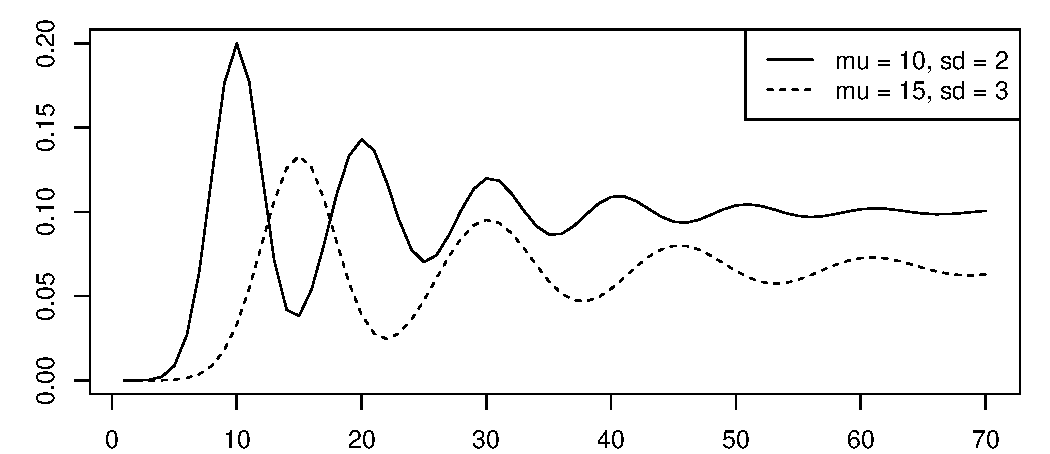
\includegraphics[width=0.40\textwidth]{images/blpa_article/pccfExamples.pdf}
    \caption{
        An example of two Gaussian PCCF functions.
        The limits are $\frac{1}{\mu^C}.$
    }
    \label{fig:pccf_example}
\end{figure}
% Local extrema of the PCCF function correspond to the time moments $l \mu, l \in \mathbb{Z}$.
% PCCF values converge to limits as defined in \Eq{eq:pccf_limit_proof} $L=1/10$ and $L=1/15$.
Prior and posteriors for the PCCF's parameters are estimated and updated using the procedure described in Section~\ref{sec:data_model} describing data model.

\section{Data model}
\label{sec:data_model}
%In~\cite{mackay2007} authors consider the general case of the Exponential family of distributions to model input data.
In this section we describe the data model which we use in BLPA.
% is the same both for input data stream of observations and for the stream of changepoints time locations.
%In BLPA method we use a particular set of probability distributions to model the data which we describe in this section.
There are two streams of data to be analysed.
The stream of input observations $\langle x_t \rangle$ and the stream of time intervals between changepoints  $\langle c_i - c_{i-1} \rangle$.
The first stream is used to detect changes and therefore to produce the second stream.
The stream of changes maybe updated by the outer sources providing additional information about time location of the changes.
E.g. there is a process running in parallel with the main detector which can run additional change-detection processes over collected data to identify locations of the changes in the past more precisely.
%
The stream of changepoints is used to predict future changepoints in order to adjust detector's settings to achieve a better performance.
% defined by the FA rate, detection delay $\delta$ and by TP rate.
%
Further, data $D$ is either input data stream of observations $\langle x_t \rangle$ or data stream of time intervals between consecutive changepoints $\langle c_i - c_{i-1} \rangle$.
In this section we describe a data model for $D$ common both for input signal and sequence of time intervals between changepoints.

Data $D$ is assumed to be generated by a Gaussian distribution with an unknown mean and variance.
We denote elements of $D$ by $\xcommon \in D$ with mean and variance $(\mucommon, \sigmacommon)$.

%\emph{I. Prior distributions.}\\
\subsection{Prior distributions.}
Following the notations in~\cite{JordanChapter9}, we use a \emph{normal-gamma} prior for $\mucommon$ and $\sigmacommon$:
%
\begin{align}
    %x_i &\sim N(\mu,\tau)~~i=1,...,n~\text{and}~\tau=1/\sigma^2\\
    \xcommon &\sim N(\mucommon,\taucommon),~~\taucommon=(1/\sigmacommon)^2\\
    \mucommon &\sim N(\muzerocommon,\kappazerocommon \taucommon)\\
    \taucommon &\sim Gamma(\alphazerocommon,\betazerocommon)
    \label{eq:theta_normal_gamma}
\end{align}
%
where $(\alphazerocommon, \betazerocommon, \muzerocommon,
\kappazerocommon)$ are hyperparameters.
%
The value $\taucommon$ is also named
\emph{precision}~\footnote{Further we use $\sigma$ and $\tau$
    parameters interchangeably.}.
%
The likelihood of data $D=\langle \xcommon \rangle$ is
%
\begin{equation}
P(D|\mucommon, \taucommon) = \Big(\frac{\taucommon}{2\pi} \Big)^{n/2}  \exp \Big (-\frac{\taucommon}{2}\sum_{i=1}^{n}(\xcommon-\mu)^2 \Big)
\end{equation}
%
The joint conjugate prior for parameters $(\mucommon,\taucommon
)$ is the defined \emph{normal-gamma} (\textit{NG}) distribution:
%
\begin{align}
    &P(\mucommon,\taucommon | \muzerocommon,\kappazerocommon,\alphazerocommon,\betazerocommon) =  N(\muzerocommon,\kappazerocommon \taucommon) Gamma(\alphazerocommon,\betazerocommon)\\
    &=\frac{1}{Z}\taucommon^{1/2}\exp\Big(-\frac{\kappazerocommon \taucommon}{2}(\mucommon-\muzerocommon)^2\Big)\taucommon^{\alphazerocommon-1}e^{-\taucommon \betazerocommon}\\
    &=\frac{1}{Z}\taucommon^{\alphazerocommon-1/2}\exp\Big(-\frac{\taucommon}{2}[\kappazerocommon(\mucommon-\muzerocommon)^2+2\betazerocommon]\Big)
\end{align}
%
where $Z=\frac{\Gamma(\alphazerocommon)}{\betazerocommon^{\alphazerocommon}}\Big(\frac{2\pi}{\kappazerocommon}\Big)^{1/2}$
is the normalized factor.

\subsection{Posterior distributions}
%Therefore,
The posterior can be derived as
%
\begin{align}
    P(\mucommon,\taucommon|D) &\varpropto P(\mucommon,\taucommon|\muzerocommon,\kappazerocommon,\alphazerocommon,\betazerocommon)P(D|\mucommon, \taucommon)\\
    &\propto N(\mucommon_n, \kappacommon_n \taucommon) Gamma(\alphazerocommon+n/2,\betacommon_n)
    \label{eq:mu_tau_posterior}
\end{align}
%
which is also a \emph{normal-gamma} distribution:
%
\begin{equation}
P(\mucommon,\taucommon|D)=NG(\mucommon,\taucommon|\mucommon_n,\kappacommon_n,\alphacommon_n,\betacommon_n)
\label{eq:mu_tau_prior}
\end{equation}
%
with the parameters
%
\begin{align}
    \mucommon_n&= \frac{\kappazerocommon}{\kappazerocommon + n} \muzerocommon + \frac{n}{\kappazerocommon + n} \bar x\\
    \kappacommon_n&= \kappazerocommon + n\\
    \alphacommon_n&= \alphazerocommon + n/2 \\
    \betacommon_n&= \betazerocommon+\frac{1}{2}\sum_{i=1}^{n}(\xcommon-\bar{x})^2+\frac{\kappazerocommon n(\bar{x}-\muzerocommon)^2}{2(\kappazerocommon+n)}
    \label{eq:update_rule}
\end{align}
%
%\begin{align}
%\mu_n&= \frac{\kappa_0}{\kappa_0 + n} \mu_0 + \frac{n}{\kappa_0 + n} \bar x\\
%\kappa_n&= \kappa_0 + n\\
%\alpha_n&= \alpha_0 + n/2 \\
%\beta_n&= \beta_0+\frac{1}{2}\sum_{i=1}^{n}(x_i-\bar{x})^2+\frac{\kappa_0 n(\bar{x}-\mu_0)^2}{2(\kappa_0+n)}
%\label{eq:update_rule}
%\end{align}
%
where $\bar{x}=\frac{1}{n}\sum_{i=1}^{n}\xcommon$ is the mean of sampled data.
% do we need this ?
The posterior distribution for $\taucommon$ is obtained by
integrating Equation~\ref{eq:mu_tau_prior} over $\mu$
(See~\cite{JordanChapter9}) --
%
\begin{multline}
    p(\taucommon | D, \muzerocommon, \kappazerocommon, \alphacommon, \betacommon) \varpropto\\
    Gamma(\alphacommon + n/2, \betacommon + \frac{1}{2} \sum_{i=1}^n (\xcommon-\bar{x})^2 +
    \frac{\kappacommon \kappazerocommon}{2(\kappacommon + \kappazerocommon)} (\bar{x} - \muzerocommon)^2 ))
    \label{eq:kappa_posterior}
\end{multline}
%
Given the updated parameters
$\theta=(\alpha_0, \beta_0, \mu_0, \kappa_0)$ using the rules~\ref{eq:update_rule} ,
the predictive distribution for a new data $x_{\text{new}}$ is
%
\begin{multline}
    p(x_{\text{new}} | \pmb{x}, \mu, \kappa, \alpha, \beta) = \\
    \int p(x_{\text{new}} | \mu, \tau) p(\tau | \pmb{x}, \mu_0, \kappa_0, \alpha, \beta) d \tau
    \label{eq:predictive_distribution}
\end{multline}
%
where
%
\begin{equation}
p(x_{\text{new}} | \mu, \tau) = (\frac{\tau}{2 \pi})^{1/2} e^{-\frac{\tau}{2} (x-\mu)^2} d \tau
\end{equation}
%
and $p(\tau | \pmb{x}, \mu_0, \kappa_0, \alpha, \beta)$ is given by~\ref{eq:kappa_posterior}.
%
Integral~\ref{eq:predictive_distribution} is a Pearson type VII distribution (Equation~\ref{eq:predictive_distribution2}) which is
equivalent of the non-standardized Student's t-distribution.
%~\cite{JordanChapter9}.
% https://en.wikipedia.org/wiki/Pearson_distribution#The_Pearson_type_VII_distribution
% The Pearson type VII distribution is equivalent to the non-standardized Student's t-distribution
\begin{equation}
p(x_{\text{new}})=\frac{1}{\alpha B(m - 1/2,1/2)} \Big (  1 + \Big (\frac{x_{n+1} - \lambda}{\alpha} \Big )^2 \Big )^{-m}
\label{eq:predictive_distribution2}
\end{equation}
%
where
%
\begin{align}
    m &= \alpha_0 + (n+1)/2\\
    %
    \alpha &= A \sqrt{ \sum_{i=1}^{n} x_i^2 + \kappa_0 \mu_0^2 - \frac{( \sum_{i=1}^{n} x_i + \mu_0 \kappa_0 )^2}{n + \kappa_0} + 2 \beta_0 }\\
    %
    A &= \sqrt{\frac{n+1+\kappa_0}{n+\kappa_0}}\\
    %
    \lambda &= \frac{\sum_{i=1}^n x_i + \mu_0 \kappa_0}{n + \kappa_0}
    \label{eq:posteriro_parameters}
\end{align}
%\alpha &= \sqrt{ \frac{n+1+\kappa_0}{n+\kappa_0} \Big ( \sum_{i=1}^{n} x_i^2 + \kappa_0 \mu_0^2 - \frac{( \sum_{i=1}^{n} x_i + \mu_0 \kappa_0 )^2}{n + \kappa_0} + 2 \beta_0 \Big)}\\
Predictive distribution~\ref{eq:bd_marginal_predictive} in case
of this data model is given by Equation~\ref{eq:predictive_distribution2}.
Please see detailed calculations in the Appendix.

\section{BLPA change detector}
\label{sec:BLPA}
% Explained in the Introduction: ?
The BLPA method is a combination of BD detector and PCCF predictive function.
Particularly when we compute the joint probability $P(r_t, \langle x_j \rangle_{j=1}^{t})$
and after that when computing the run-length distribution
$P(r_t | \langle x_j \rangle_{j=1}^{t})$
we multiply these probabilities by the prior probability of the
changes given by PCCF for the moment $t$.
%
The BLPA method is depicted in Algorithm~1, %\ref{alg:pccf_detector}
in which:
%
\begin{itemize}
    \item Lines 1-4: Set initial parameters values for the probability distribution of the data $D$.

    \item Line 5: Compute PCCF using initial values of the
        parameters (Equation~\ref{eq:pccf}).

    \item Line 7: Collect a new measurement.

    \item Line 8: Compute predictive distribution using Equation~\ref{eq:predictive_distribution2}.

    \item Line 9-10: Compute change probabilities and `growth' probabilities of the run length.

    \item Line 11: Compute posterior probabilities of run lengths (changes).

    \item Line 12: Update parameters of the probability distributions for the data $D$ using Equations~\ref{eq:update_rule}.

    \item Lines 13-16: Find the most likely position of the last changepoint, update PCCF parameters and recalculate PCCF.
\end{itemize}

\input{./parts/PseudoCodeDetector.tex}

\section{Experiments}
\label{sec:experiments}
We performed experiments with artificially generated and real
data sets.
% === START: MOVE TO EXPERIMENTS SECTION
To measure the performance of the change detector we can consider it as as a binary classifier assigning labels `change'/`not change' to the incoming observations $x_t$.
If
$\Event{t}{+}$ is the `change' label assigned at the moment $t$
and
$\Event{t}{-}$ is the label `not change' assigned at $t$
then
Then True Positive (TP), False Positives (FP), True Negatives (TN) and False Negatives (FN) events can be defined as follows:
\begin{itemize}[leftmargin=*]\setlength\itemsep{0em}
    \item $\Event{t}{+}$ is TP if $\exists c_i:t-c_i<\delta$, and FP if $\nexists c_i:t-c_i<\delta$
    \item $\Event{t}{-}$ is FN if $\exists c_i:t-c_i <\delta$, and TN if $\nexists c_i:t-c_i<\delta$
\end{itemize}
The \textit{performance of the change detector} is defined by TP/FP rates and by the average delay $\delta$ of the detection.
% === END: MOVE TO EXPERIMENTS SECTION

\subsection{Artificial data}
In the simulation we generated 200 signals with 10 recurrent changes in the mean value for each hazard-rate value $h$ varied in the interval from 50 to 300 by the step 15.
%While changing the hazard-rate parameter $h$ from the value 50 to 300 by the step 200 signals were generated for each $h$.
%Sensitivity parameter of the detector was variated from 50 to 300 by the step 15
Average distance between changes was set to $\mu = 100$ with the standard deviation $\sigma = 10$.
%
%Number of changes in each signal is $10$.
Results are depicted in Fig.~\ref{fig:results1}.
%\input{AllFigures.tex}
\input{FigResults1.tex}
FP rate is decreased while not reducing TP rate.
In the worst cases the performance of both detectors is similar.

\subsection{Human Activity (HA) signal}
%https://archive.ics.uci.edu/ml/datasets/Smartphone-Based+Recognition+of+Human+Activities+and+Postural+Transitions
In the second experiment we used the Human activity data set~\cite{reyes2016transition} which contains sensor measurements from people performed 6 types of activities: three static postures (standing, sitting, lying) and three dynamic activities (walking, walking downstairs and walking
upstairs).
We detected changes in the signal caused by transitions from one set activities to another.
Results are depicted in Fig.~\ref{fig:results2}.
\input{FigResults2.tex}
FP rate is decreased when BD detector is used with the PCCF function.


\section{Conclusion}
We proposed the method to improve performance of the Bayesian Online Changepoint detector (BD) for the data streams with recurrent changes by embedding into it the Predictive Confidence Change Function (PCCF).
%
While observing a new data both BD detector's and PCCF's parameters are adjusted in a uniform way to the changing conditions using the same Bayesian update procedures constituting a two-layer adaptive change detection/prediction method BLPA.
%
In the experiments with real and artificial data sets we demonstrated that Bayesian detector equipped with PCCF performs better in terms of TP/FP rates than the detector without PCCF.
%We extended the method proposed in~\cite{mackay2007} by
%\bibliographystyle{IEEEtran}
%\input{./parts/Appendix}
\appendix
\noindent
\textbf{Marginal predictive distribution} $p(x_{n+1}|x_1,...,x_n)$ can be found as
\begin{align}
\label{eq:post1}
    &p(x_{n+1}|x_1,...,x_n)\\\nonumber
    &=\frac{ \int_{\tau\in \mathbb{R}^+} \int_{\mu\in \mathbb{R}}p(x_1,....,x_{n+1}|\mu,\tau) p(\mu,\tau)d\mu d\tau}{ \int_{\tau\in \mathbb{R}^+} \int_{\mu\in\mathbb{R}}p(x_1,....,x_{n}|\mu,\tau) p(\mu,\tau)d\mu d\tau}.
\end{align}
Assuming the Gaussian distribution 
\begin{equation}
    p(x|\mu,\tau)=\frac{\sqrt{\tau}}{\sqrt{2\pi}} e^{-\frac{\tau}2 (x-\mu)^2}
    \label{eq:gauss_appendix}
\end{equation}
the probability $p(x_1,....,x_{n}|\mu,\tau) p(\mu,\tau)$ is
\begin{align}\label{eq:prob1}
    \left(\frac{\sqrt{\tau}}{\sqrt{2\pi}}\right)^{n}\times &\exp\left(-\frac{\tau}{2}\sum_{i=1}^{n} (x_i-\mu)^2\right) \tau^{\alpha_0-1/2}\\\nonumber &\times\exp\left(-\frac{\tau}2 \left(\kappa_0(\mu-\mu_0)^2+2\beta_0\right) \right)
\end{align}
where an expression in the exponent is 
\begin{align}
    &-\frac{\tau(n+\kappa_0)}{2}\sum_{i=1}^{n} \left(\mu-\frac{\sum_{i=1}^{n} x_i+\mu_0 \kappa_0}{n+\kappa_0}\right)^2\\\nonumber &-\frac{\tau}{2} \left(\sum_{i=1}^{n} x_i^2 + \kappa_0\mu_0^2 - \frac{(\sum_{i=1}^{n}x_i +\mu_0 \kappa_0)^2}{n+\kappa_0}+2\beta_0\right),
\end{align}
Therefore %from where
\begin{align}
    &p(x_1,....,x_{n}|\mu,\tau) p(\mu,\tau)\\\nonumber
    =& \left(\frac{1}{\sqrt{2\pi}}\right)^{n-1} \frac{\Gamma(\alpha_0+n/2)}{\sqrt{n+\kappa_0}} \left(\frac{\hat{b}_n}2\right)^{-\alpha_0+n/2}\\\nonumber \times &\GammaDistr(\tau|\alpha_0+n/2,\hat{a}_n/2) \mathcal{N}(\mu|\hat{\mu}_n,\hat{\sigma}^2_n)
\end{align}
where posterior parameters estimates $\hat{a}_n, \hat{\mu}_n, \hat{\sigma}^2_n$ are
\begin{align}
    &\hat{a}_n = \left(\sum_{i=1}^{n} x_i^2 + \kappa_0\mu_0^2 - \frac{(\sum_{i=1}^{n}x_i +\mu_0 \kappa_0)^2}{n+\kappa_0}+2\beta_0\right),\\\nonumber &\hat{\mu}_n = \frac{\sum_{i=1}^{n}x_i+\mu_0 \kappa_0}{n+\kappa_0},\ \hat{\sigma}^2_n = \frac{1}{\tau(n+\kappa_0)}.
\end{align}
Therefore the integral in the numerator in Equation~\ref{eq:post1} is
\begin{align}
    &\int_{\tau\in \mathbb{R}^+} \int_{\mu\in \mathbb{R}}p(x_1,....,x_{n+1}|\mu,\tau) p(\mu,\tau)d\mu d\tau\\\nonumber
    =& \left(\frac{1}{\sqrt{2\pi}}\right)^{n-1} \frac{\Gamma(\alpha_0)}{\sqrt{n+\kappa_0}} \left(\frac{\hat{a}_n}2\right)^{-(\alpha_0+n/2)}
\end{align}
and integral~\ref{eq:post1} can be expressed as
\begin{align}
    &\frac{\sqrt{n+\kappa_0}}{\sqrt{n+1+\kappa_0}\ B(\alpha_0+n/2,1/2)} \frac{\hat{a}_n^{\alpha_0+n/2}}{\hat{a}_{n+1}^{\alpha_0+(n+1)/2}}\\\nonumber
    =&\frac{\sqrt{n+\kappa_0}}{\sqrt{n+1+\kappa_0}\ B(\alpha_0+n/2,1/2)} \left(\frac{\hat{a}_{n+1}}{\hat{a}_n}\right)^{-(\alpha_0+(n+1)/2)} \hat{a}_n^{-1/2}.
\end{align}
Noticing that
\begin{align}
    &\frac{\hat{a}_{n+1}}{\hat{a}_n} = 1+ \frac{n+\kappa_0}{\hat{a}_n(n+1+\kappa_0)}\\\nonumber \times &\left(x_{n+1}^2 - \frac{2x_{n+1}\left(\sum_{i=1}^n x_i +\mu_0 \kappa_0\right)}{n+\kappa_0}
    + \frac{\left(\sum_{i=1}^n x_i +\mu_0 \kappa_0\right)^2}{(n+\kappa_0)^2}\right)
\end{align}
\textbf{marginal predictive distribution} is 
\begin{align}
    &p(x_{n+1}|x_1,...,x_n)\\\nonumber =& \frac{1}{\hat{b}_n B(\alpha_0+n/2,1/2)} \left(
1+\frac{(x_{n+1}-\lambda)^2}{\hat{b}_n^2}\right)^{-(\alpha_0+(n+1)/2)},
\end{align}
where coefficients are
\begin{equation}
    \hat{b}_n = \frac{\sqrt{(n+1+\kappa_0)\hat{a}_n}}{\sqrt{(n+\kappa_0)}},\ \lambda = \frac{\sum_{i=1}^n x_i +\mu_0 \kappa_0}{n+\kappa_0}.
\end{equation}

